\chapter{Definitions}
\label{chap:definitions}
This work proposes the application of a high availability technique to a context broker system. For a better understanding of the system and its development, definitions of Context, Context-Aware System, Context Representation, Fault Tolerance and High Availability related terms are presented.

\section{Context}
\label{sec:context}

Context has had many definitions throughout the years. The first time Context was defined regarding the human-computer interaction was by \cite{schilit1994disseminating}, where context is defined related to location, identities of nearby people and objects, and the changes happening to those.  Similarly, \cite{brown1997context} define context as location, people around the user, time of day, season, temperature, etc. Many authors have also defined context using synonyms, as \cite{brown1995stick} had the idea of “environment”, i.e., what the computer knows about the user's environment, or \cite{franklin1998all} that see context as the user's situation. Thus, a lot of definitions have existed, but they all end up being too specific. Context is about the whole situation of an application and its users, and we can't really define it as being too specific to something like a location, or the environment a user is in.

Therefore, the definition of context made by \cite{dey2000providing} is as follows: ''Context is any information that can be used to characterize the situation of an entity. An entity is a person, place, or object that is considered relevant to the interaction between a user and an application, including the user and application themselves.'' This is the definition this work uses.

\subsection{Context-Aware System}
Like context, context-awareness has had several definitions over the years. The first definition was done by \cite{schilit1994disseminating}, and it restricted to applications informed about context and applications that adapt themselves to context. Later on, synonyms have been used to define a context-aware system: reactive \cite{cooperstock1995evolution}, responsive \cite{elrod1993responsive}, situated \cite{hull1997towards}, context-sensitive  \cite{rekimoto1998augment} and environment-directed \cite{fickas1997software}. All these definitions refer to either using or adapting to context, however, a more global definition is needed, covering every interaction with context made by the system.

The definition used in this work is provided by \cite{dey2000providing}: ''A system is context-aware if it uses context to provide relevant information and/or services to the user, where relevancy depends on the user's task.''

\todo{(talk briefly about Provider and Consumer, and why to use a Broker)}

\subsection{How to represent Context}
According to \cite{dey2000providing}, context-aware applications deal with the who's, where's, when's and what's (the activities that are occurring) of entities, and interpret this information to define why a situation is occurring. Then, the designer of the application must decide what to do with the information. Once we have the information available, either through automated sensors or through user's interference, we need to represent it in a way a machine can process and store it.

\cite{baldauf2007survey} presents and defines the most relevant context modeling options: key-value, markup scheme, graphical, object oriented, logic based and ontology based models. As this work is developed following the same core as \cite{crippa2010}, it uses the same context representation model: a markup scheme variation, \textbf{ContextML} \cite{knappmeyer2010contextml}. The network nature of the messages (HTTP messages, in this case) facilitates textual, non graphic model. 

\subsection{ContextML}

ContextML is an XML-based representation schema for context information, where it is categorized into scopes and related to different types of entities. It is designed to be used with REST-based communication between the framework components \cite{knappmeyer2010contextml}. It was created within a project called C-CAST \cite{ccast}, a collaborative work of many companies, research centers and universities, and its main objective is to evolve mobile multimedia multicasting to exploit the increasing integration of mobile devices with our everyday physical world and environment \cite{crippa2010}. The architecture of the system presented in this work is based on the architecture of the C-Cast Project system.

The system consists on three core components: \textbf{Context Provider}, \textbf{Context Consumer} and \textbf{Context Broker}. They are briefly described below, based on definitions made by \cite{knappmeyer2010contextml}. 

\subsubsection{Context Provider}
A \textbf{Context Provider} (CxP) provides context information of a certain type, e.g. weather, location, activity, etc. It gathers data from sensors, network, user interactions, or other sources. A CxP is specialized in a specific domain of context information (location, weather etc).


\subsubsection{Context Consumer}
A \textbf{Context Consumer} (CxC) queries for and uses context data, e.g. is a context-aware application. A CxC can retrieve context information asynchronously through a subscription method, or by a synchronous method where it requests the Broker for a specific information or for a particular Provider interface, to query the Provider directly.

\subsubsection{Context Broker}
A \textbf{Context Broker} (CxB) is the central component of the architecture, and is the focus of this work. It handles and aggregates context information, and is an interface between the other architecture components. The CxB allows CxCs to subscribe to context information, and CxPs to provide this information. It also provides a lookup service, where the CxCs can query the CxB for CxPs that have a particular capability, depending on the CxC’s interest.

\subsubsection{Entity and Scope}
An entity is the subject of interest which context data refers to, and it is composed of two parts: a type and an identifier. The type refers to the category of the entity: username for human users, imei for mobile devices, room for a room with sensors, etc. The identifier specifies a particular item within a set of entities of the same type.

A scope is a set of closely related context parameters. Every context parameter has a name and belongs to only one scope. The parameters of a scope can only be requested, updated, provided and store at the same time, making the data always consistent. For example, a scope \textit{position} has latitude, longitude and accuracy attributes; any operation on this scope is performed on all these attributes: if the latitude is updated, so is the longitude and accuracy, what is correct, because otherwise it would not make sense. Entity-scope association is illustrated in Figure \ref{fig:entityscope}. \par

\begin{figure}[H]
	\centering
	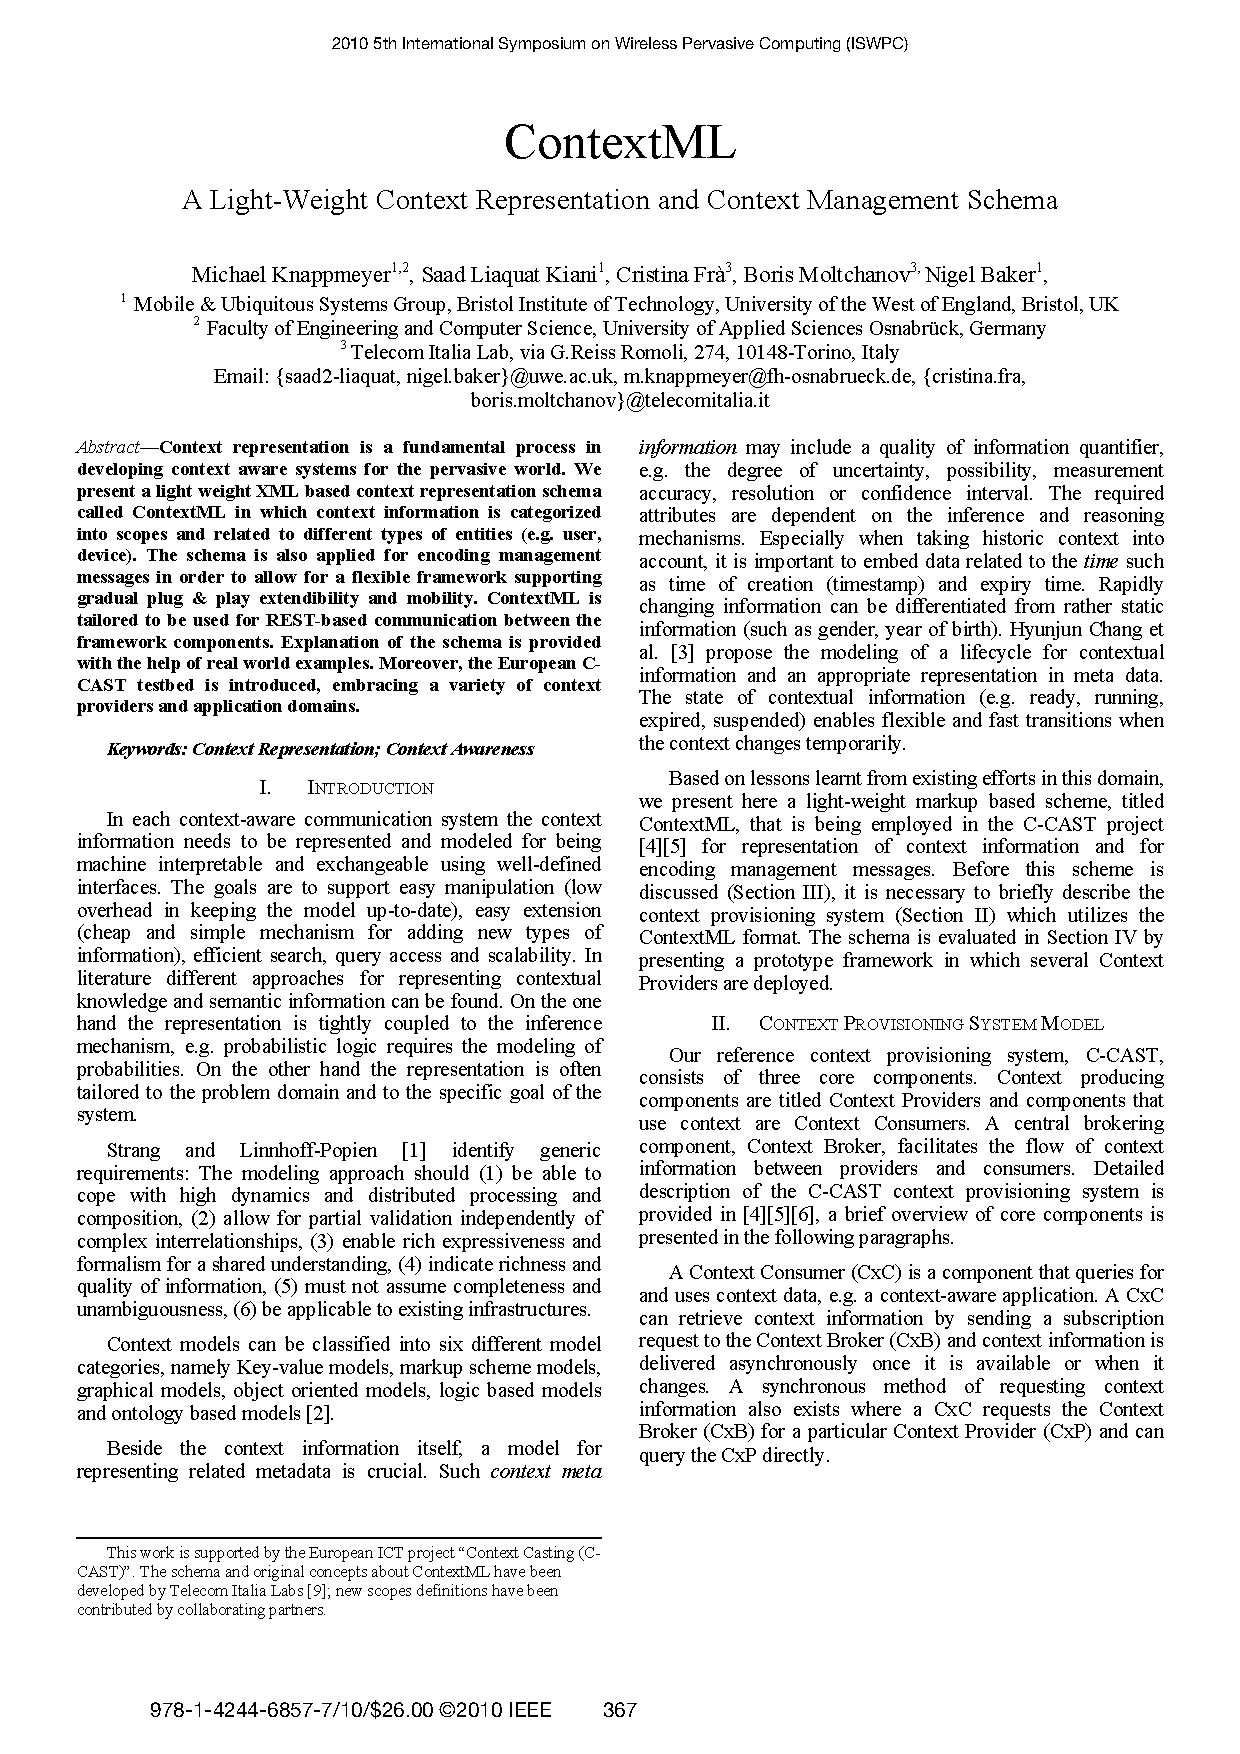
\includegraphics[scale=1]{entityscope.pdf}
	\caption{Entity and Scope relationship. Source: \cite{knappmeyer2010contextml}}
	\label{fig:entityscope}
	
\end{figure}

\subsubsection{ContextML Messages}
Within the architecture of the system, context is registered, updated and queried following a set of pre-defined ContextML messages, that follow the proposed by \cite{knappmeyer2010contextml}. The possible ContextML messages and their uses are shown below, as well as a simple example of each one.

\begin{description}
\item[Advertisement Message]\hfill \\
An Advertisement Message is used by the Context Provider to register its capabilities to the broker. It informs the CxP’s access url (urlRoot), what scopes it supports (scopes), its identifier (name), and optional information about the CxP’s location. An example of a Advertisement Message can be seen in Figure \ref{fig:advertisement}.

\begin{figure}[H]
	\centering
	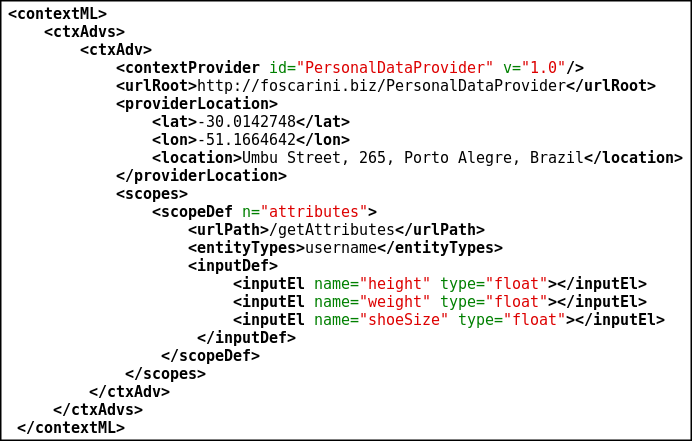
\includegraphics[scale=0.5]{advertisement.png}
	\caption{Provider Advertisement example message}
	\label{fig:advertisement}
	
\end{figure}

\item[CxP Lookup Message]\hfill \\
When a CxC wants to know where it can find a specific scope, it can query the CxB about which of the registered Providers has the desired information. The Broker replies with a ContextML message, describing the Providers that match with the data required by the CxC. An example can be seen in Figure \ref{fig:providers}.

\begin{figure}[H]
	\centering
	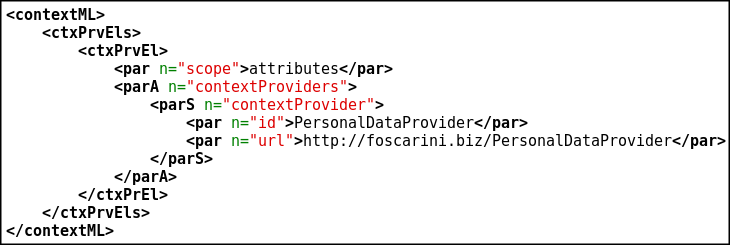
\includegraphics[scale=0.5]{providers.png}
	\caption{Providers Lookup example message}
	\label{fig:providers}
	
\end{figure}

\item[ACK Message]\hfill \\
Acknowledgement is a control message that confirms the execution of various management actions (e.g. advertisement, context update). Each ACK message contains the status of the operation, the HTTP response code, and the identification of the method it corresponds. It also has optional fields to inform scope and entity information. An example is shown in Figure \ref{fig:acknack}.

\begin{figure}[h]
	\centering
	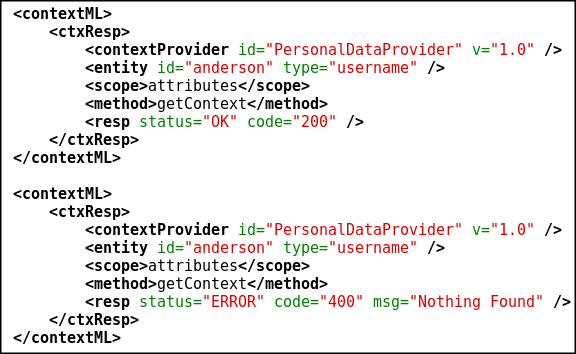
\includegraphics[scale=0.5]{acknack.png}
	\caption{ACK and NACK example messages}
	\label{fig:acknack}
	
\end{figure}


\item[Context Representation Message]\hfill \\
When a Consumer requests or subscribes to a context scope, it receives a ContextML message with the element \textit{‘ctxEl’}, when the information queried is available. \textit{ctxEl} contains information of the provider that has the context queried (contextProvider), the entity and scope it is related to, and the context data in the \textit{dataPart} element. \textit{par}, \textit{parS} and \textit{parA} are constructors to store name-value pairs and attribute collections (structs and arrays) respectively. Every context information that is exchanged is tagged with a \textit{timestamp} (time of its generation) and an expiration time \textit{expires} (validity of the context information), after which the information is considered invalid. An example of a Context Representation Message is shown in Figure \ref{fig:ctxels}.

\begin{figure}[h]
	\centering
	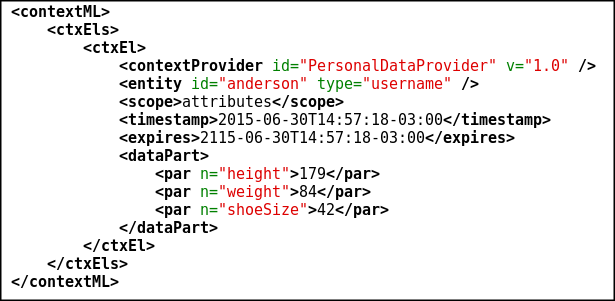
\includegraphics[scale=0.5]{ctxels.png}
	\caption{Context Element example messages (update)}
	\label{fig:ctxels}
	
\end{figure}


\end{description}


\section{Dependability}
\label{sec:fault_tolerance}

According to \cite{avivzienis2004basic}, the dependability of a system is the ability to avoid service failures that are more frequent and more severe than is acceptable, i.e., failures will eventually happen, and the system will try to avoid them compromising the correctness of the service. Dependability is an integrating concept that encompasses the following attributes:
\begin{itemize}
	\item{Availability:} readiness for correct service
	\item{Reliability:} continuity of correct service
	\item{Safety:} absence of catastrophic consequences on the user(s) and the environment
	\item{Integrity:} absence of improper system alterations
	\item{Maintainability:} ability to undergo modifications, and repairs
\end{itemize}
\subsection{Fault Tolerance}
As seen on \cite{avivzienis2004basic}, many means can be developed to attain the various attributes of
dependability and security. Those means can be grouped into four major categories:
\begin{itemize}
	\item{Fault Prevention} means to prevent the occurrence or introduction of faults
	\item{Fault Tolerance} means to avoid service failures in the presence of faults
	\item{Fault Removal} means to reduce the number and severity of faults
	\item{Fault Forecasting} means to estimate the present number, the future incidence, and the likely consequences of faults
\end{itemize}

Fault prevention and fault tolerance aim to provide the ability to deliver a service that can be trusted. This work focuses on \textbf{fault tolerance}, which is aimed at failure avoidance, and is carried out via error detection and system recovery.



\subsection{High Availability}
On the verge of creating a fully Dependable Broker, that covers every attribute cited in the previous section, this work takes a first step, focusing on High Availability.
(give some examples of high availability in the real world, as with a temperature sensors for fire prevention, or movement sensors on a mountain that track mudslides, etc)



\subsubsection{Problems involving High Availability}
\todo{...fill me...}

\section{Proposed Idea}
The idea is to use properties of Cluster systems to structure the Dependable Broker system. For that, basic definitions needed to build the complete understanding of the system are presented.
(explain the whole idea, of how to control database changes, based on ideas on the referred articles, treat Brokers as a Cluster System, using a non-blocking commit protocol)
\cite{arsanjani2004service} \cite{barreradesign}  \cite{skeen1981nonblocking} 

